% Options for packages loaded elsewhere
\PassOptionsToPackage{unicode}{hyperref}
\PassOptionsToPackage{hyphens}{url}
%
\documentclass[
  14pt,
]{book}
\title{Governing Documents Amberson Towers Condominums}
\author{}
\date{\vspace{-2.5em}Last Association Revision: October 13, 2021; Last Draft Build: February 15, 2020}

\usepackage{amsmath,amssymb}
\usepackage{lmodern}
\usepackage{iftex}
\ifPDFTeX
  \usepackage[T1]{fontenc}
  \usepackage[utf8]{inputenc}
  \usepackage{textcomp} % provide euro and other symbols
\else % if luatex or xetex
  \usepackage{unicode-math}
  \defaultfontfeatures{Scale=MatchLowercase}
  \defaultfontfeatures[\rmfamily]{Ligatures=TeX,Scale=1}
\fi
% Use upquote if available, for straight quotes in verbatim environments
\IfFileExists{upquote.sty}{\usepackage{upquote}}{}
\IfFileExists{microtype.sty}{% use microtype if available
  \usepackage[]{microtype}
  \UseMicrotypeSet[protrusion]{basicmath} % disable protrusion for tt fonts
}{}
\makeatletter
\@ifundefined{KOMAClassName}{% if non-KOMA class
  \IfFileExists{parskip.sty}{%
    \usepackage{parskip}
  }{% else
    \setlength{\parindent}{0pt}
    \setlength{\parskip}{6pt plus 2pt minus 1pt}}
}{% if KOMA class
  \KOMAoptions{parskip=half}}
\makeatother
\usepackage{xcolor}
\IfFileExists{xurl.sty}{\usepackage{xurl}}{} % add URL line breaks if available
\IfFileExists{bookmark.sty}{\usepackage{bookmark}}{\usepackage{hyperref}}
\hypersetup{
  pdftitle={Governing Documents  Amberson Towers Condominums},
  hidelinks,
  pdfcreator={LaTeX via pandoc}}
\urlstyle{same} % disable monospaced font for URLs
\usepackage{longtable,booktabs,array}
\usepackage{calc} % for calculating minipage widths
% Correct order of tables after \paragraph or \subparagraph
\usepackage{etoolbox}
\makeatletter
\patchcmd\longtable{\par}{\if@noskipsec\mbox{}\fi\par}{}{}
\makeatother
% Allow footnotes in longtable head/foot
\IfFileExists{footnotehyper.sty}{\usepackage{footnotehyper}}{\usepackage{footnote}}
\makesavenoteenv{longtable}
\usepackage{graphicx}
\makeatletter
\def\maxwidth{\ifdim\Gin@nat@width>\linewidth\linewidth\else\Gin@nat@width\fi}
\def\maxheight{\ifdim\Gin@nat@height>\textheight\textheight\else\Gin@nat@height\fi}
\makeatother
% Scale images if necessary, so that they will not overflow the page
% margins by default, and it is still possible to overwrite the defaults
% using explicit options in \includegraphics[width, height, ...]{}
\setkeys{Gin}{width=\maxwidth,height=\maxheight,keepaspectratio}
% Set default figure placement to htbp
\makeatletter
\def\fps@figure{htbp}
\makeatother
\usepackage[normalem]{ulem}
% Avoid problems with \sout in headers with hyperref
\pdfstringdefDisableCommands{\renewcommand{\sout}{}}
\setlength{\emergencystretch}{3em} % prevent overfull lines
\providecommand{\tightlist}{%
  \setlength{\itemsep}{0pt}\setlength{\parskip}{0pt}}
\setcounter{secnumdepth}{5}
\usepackage{booktabs}
\ifLuaTeX
  \usepackage{selnolig}  % disable illegal ligatures
\fi
\usepackage[]{natbib}
\bibliographystyle{plainnat}

\begin{document}
\maketitle

{
\setcounter{tocdepth}{1}
\tableofcontents
}
\hypertarget{section}{%
\chapter*{}\label{section}}
\addcontentsline{toc}{chapter}{}

\hypertarget{three-documents-define-governance}{%
\section*{Three Documents Define Governance}\label{three-documents-define-governance}}
\addcontentsline{toc}{section}{Three Documents Define Governance}

The governing documents of Amberson Towers comprise three separate documents:

\begin{itemize}
\item
  \textbf{The Rules and Regulations} - General rules which can be amended by a majority vote of the Council. Last amended in approximately September 2018.
\item
  \textbf{The Declaration} - Mostly detailed information about the building, such as surveyor's coordinates and voting share of each unit. Takes precedence over other documents. Requires agreement of 60\% owners to amend. First filed on March 14, 1978 and amended twice, most recently September 12, 1978, but only with very minor changes.
\item
  \textbf{The Code of Regulations} - Regulates how the building is governed, for example how Council is elected. Requires agreement of 60\% ow owners to amend. First filed April 12, 1978 and has been amended seven times (September 1978, 1990, 1994, 1996, 2000, 2016, and 2017).
\end{itemize}

Provided in \protect\hyperlink{documents}{Appendix A} are links to source doxcuments for \emph{The Declaration} and \emph{The Code of Regulations}.

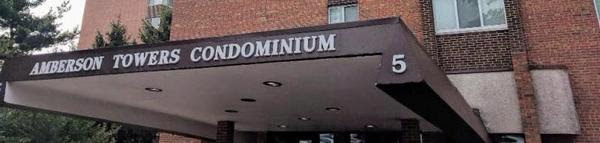
\includegraphics{amber3.jpg}

\begin{center}\rule{0.5\linewidth}{0.5pt}\end{center}

\begin{quote}
\textbf{Notes \& Disclaimer:} This publication has been produced for the convenience of our residents and users. It is an unofficial reproduction of the original documents and any amendments thereto. This version of the Code of Regulations integrates all revisions into one consolidated document. The official recorded documents should be consulted for all interpretations and applications. They are the primary source and documents for all purposes. Copies of the official documents may be inspected and obtained in the Meyers Management office. In the event of an error, misprint, omission, or conflict between the within versions and the official documents, the official printed and recorded documents shall govern and be controlling.
\end{quote}

\hypertarget{amberson-towers-condominums-rules-regulations}{%
\chapter*{\texorpdfstring{\textgreater\textgreater{} 1. Amberson Towers Condominums Rules \& Regulations}{\textgreater\textgreater{} 1. Amberson Towers Condominums   Rules \& Regulations}}\label{amberson-towers-condominums-rules-regulations}}
\addcontentsline{toc}{chapter}{\textgreater\textgreater{} 1. Amberson Towers Condominums Rules \& Regulations}

\emph{5 Bayard Road, }
\emph{Pittsburgh, Pennsylvania 15213}

\begin{center}\rule{0.5\linewidth}{0.5pt}\end{center}

The Amberson Towers Condominium Council is responsible for the operation of the Condominium. Pursuant to its Code of Regulations, the Council shall from time to time issue rulings, regulations, and conditions which shall be binding upon all Apartment Unit owners and occupants which rulings, regulations and conditions shall be in the Council's sole judgement for the general well-being, safety, care, and cleanliness of the building.

\hypertarget{i.-information-assistance}{%
\section*{I. Information \& Assistance}\label{i.-information-assistance}}
\addcontentsline{toc}{section}{I. Information \& Assistance}

A. The Property Manager is available to give unit owners information and assistance in keeping with his duties to the condominium. Such requests should be confined to regular hours except in an emergency.

B. Service requests and complaints regarding the service of the building shall be made in writing and placed in the Service boxes in the lobby or mail room.

\hypertarget{ii.-party-room}{%
\section*{II. Party Room}\label{ii.-party-room}}
\addcontentsline{toc}{section}{II. Party Room}

A. The party room is available only to unit owners for private parties. Arrangements for its use are to be made with the Property Manager on a first come, first serve basis.

B. A deposit is required for the use of the party room. It will be refunded provided that the room has been restored to its original condition.

C. The party room shall not be used for commercial purposes.

\begin{enumerate}
\def\labelenumi{\arabic{enumi}.}
\item
  Damage to the party room is the financial responsibility of the unit owner reserving it.
\item
  Tenants may use the party room providing they obtain written authorization from their unit owner, who shall be financially responsible for damage caused by them.
\end{enumerate}

\hypertarget{iii.-laundry}{%
\section*{III. Laundry}\label{iii.-laundry}}
\addcontentsline{toc}{section}{III. Laundry}

A. Laundry work shall be done only in the areas provided for such purposes.

\hypertarget{iv.-storage-lockers}{%
\section*{IV. Storage \& Lockers}\label{iv.-storage-lockers}}
\addcontentsline{toc}{section}{IV. Storage \& Lockers}

A. The Condominium Association assumes no liability for any loss or damage to articles in any common or other storage area, except where due to negligence of the Condominium Association.

B. The lobby, stairways, and other public areas shall not be used for the storage or placement of furniture or any other articles, including, but not limited to plants, boxes, etc.

C. Each unit owner is entitled to a locker in one of the storage rooms.

D. Extra storage lockers located on each floor may be rented on a monthly basis when available.

\hypertarget{v.-sound-problems}{%
\section*{V. Sound Problems}\label{v.-sound-problems}}
\addcontentsline{toc}{section}{V. Sound Problems}

A. Each unit shall be carpeted in an amount equal to 80\% of the floor space in every room, corridor, foyer, and/or vestibule with the exception of the kitchen and bathrooms.

B. No owner or occupant shall make or permit any disturbing noises to be made in the building or on the premises by himself, his family, friends, tenants, servants, or other invitees; nor permit anything to be done by such persons that would interfere with the rights, comforts or convenience of their owners or occupants.

C. No owner or occupant shall play or allow to be played any musical instrument, radio, TV, hi-fi, tape recorder or the like in the premises between the hours of 11 :00 pm and the following 8:00 am if the same shall disturb or annoy other owners or occupants of the building.

\hypertarget{vi.-garage}{%
\section*{VI. Garage}\label{vi.-garage}}
\addcontentsline{toc}{section}{VI. Garage}

A. No major automobile or vehicle repairs are permitted on any part of the premises. Emergency repairs and seasonal tire changes are permitted. Car washing is not permitted.

B. Council shall have the authority to reassign parking spaces in extreme hardship cases or in cases where such a redistribution may lead to more efficient use of the space, i.e.~small cars may be assigned to smaller spaces than large cars.

C. Cars parked in spaces assigned to others will be towed away at the expense of the violator, unless prior permission has been obtained from the person to whom the spaces are assigned.

D. All shopping carts shall be returned to the storage rooms on the IP, 2P, and 3P levels of the garage from where they were taken after use.

E. Parking garage spaces shall be available only to resident unit owners or occupants on an annual basis.

F. Parking garage spaces shall be allocated on the basis of the following priorities: First priority: first car of unit owner in residence; second priority: first car of tenant; third priority: second car of unit owner in residence; fourth priority second car of tenant. These spaces cannot be sublet.

G. Any resident who is planning not to occupy his or her garage space for a continuous period of one month or more, shall notify the management office so that the space can be reassigned for that period based upon the priority list. Any resident who so notifies the management office will not be charged garage rent for the period of his or her absence during which the management office is able to reassign the space.

H. Idling of vehicles, engine or leaving them unattended with the engine running in the garage is prohibited. Violations of this provision are subject to double the fines listed in Article IX hereof.

I. Unit owners parking in the Amberson Towers garage who are delinquent in their monthly maintenance fees or parking fees by more than one month will lose their right to park in the garage. This will include tenants of owners who are delinquent in paying their fees.

J. Garage renters who are to lose their parking space because they are delinquent will be notified ten days in advance before any action is taken. Persons losing a parking space are not guaranteed a subsequent parking space if the garage is fully occupied. Their names will be placed on a waiting list behind others already on the list.

\hypertarget{vii.-security-keys}{%
\section*{VII. Security \& Keys}\label{vii.-security-keys}}
\addcontentsline{toc}{section}{VII. Security \& Keys}

A. The security system is for the protection of all unit owners. To be fully effective, this system requires that outsiders gain entrance to the building only upon the authorization of the unit owner whom they are visiting.

B. The key to any door shall not be loaned or given to a domestic or attendant unless such person lives in the building.

C. Unit Owners or occupants must not open any entry door for persons whom they do not know.

\protect\hyperlink{Sect4D}{D.} The Property Manager must retain a passkey to each unit. No unit owner shall alter any lock or install a new lock on any door leading to his or her unit unless the owner shall provide the management with a key for management's use.

E. Except as required in \protect\hyperlink{Sect4D}{section D} above, the unit owner accepts responsibility for any damages resulting as a consequence of keys entrusted by him or his designated agent to any employee pf the Condominium Association.

F. No keys to any unit shall be left in the management office without notice to and acceptance by office management, and no keys shall be left to be given to any person other than an owner to that unit.

\hypertarget{viii.-general}{%
\section*{VIII. General}\label{viii.-general}}
\addcontentsline{toc}{section}{VIII. General}

A. Nothing shall be done or kept in any unit in the common elements which will increase the rate of insurance of the building or contents thereof applicable for residential use without the prior consent of the Council.

B. Nothing shall be thrown or emptied by the owners or their tenants or servants out of the window or doors, or down the stairways, or in the common areas, nor sh.all anything be hung from outside of the window sills.

C. No occupant shall interfere in any manner with any portion either of the heating or electrical apparatus in or about the building.

D. The addition of any major appliance, such as frost-free refrigerators, convection ovens, and room-sized humidifiers, shall require approval of Council. Washers and dryers, electric ranges, and window air conditioners are not permitted.

E. No awnings or window guards shall be installed except as shall be put up or approved by the Council and no signs of any kind shall be placed in windows or on doors or on the exterior surfaces or common elements without prior written approval of the Council.

F. All unit owners shall provide white curtain liners or white glass curtains as are presently used in the building.

G. No radio or TV aerial shall be installed by the occupants outside of their respective units.

H. No occupants or owners of the building shall send any employee of the Condominium Association out of the building on any private business.

I. No unit owner or any of his agents, servants, employees, licensees, or visitors shall at any time bring into or keep in his unit any flammable, combustible, or explosive substance, except for normal household use.

J. No solicitations shall be conducted on the premises without written consent of the Council.

K. Water beds shall not be installed or used in any apartments.

L. Owners shall not be permitted to put their names in any entry, passageway, vestibule, hall or stairway of the building, except in the proper place or on the mailbox provided for use of the units occupied by them respectively.

M. No rugs shall be beaten on patios, outdoor living areas, stairways, halls or corridors; nor shall dust, rubbish, or litter be swept from unit, into any of the halls ·or entryways of the building.

N. Use of the roofs shall be confined to the deck areas. Grilling on the roof is prohibited.

O. Children shall not be permitted to loiter or play on the stairways or in the halls, lobbies, elevators, parking ramps, or any other common areas except for the lawns, the terrace or private patios, with permission of the owner holding the easement for such patio.

P. The water closets, laundry rooms, and other water apparatus will not be used for any purpose other than that for which they were constructed , and no rubbish, rags or papers shall be thrown therein. Any damage to the property or unit of others, including the common elements, resulting from misuse of such facilities or the negligence of the unit owner or occupant shall be paid for by the owner of the unit in which such misuse occurred.

Q. Any damage to the premises caused by the moving and/or carrying of articles therein shall be paid for by the owner of such articles. All large-scale moving must be arranged with the management office. Moving, delivery or carrying of furniture, appliances or any large items through the lobby of the building is prohibited.

R. No animals, birds or pets of any kind shall be brought or kept in or about the apartment unit or the building.

S. All Unit Owners establishing a new lease or extending the present lease are required to make the Amberson Towers Rules and Regulations a part of that lease.

T. Each Unit owner shall carry an apartment owner's comprehensive insurance policy covering the inside of his apartment for contents

U. No unit owner or occupant shall conduct a public, estate or yard sale of furniture or other personal belongings in the building. Signs, notices, and messages of any kind shall be restricted to the bulletin boards in the mail room. Political signs, notices, advertisements or messages are not permitted.

V. Prospective buyers must be confined to the seller's unit.

W. Any consent or approval given under these Rule and Regulations may be added to, amended or repealed at any time by resolution of the Council.

X. In addition to the alternative procedure set out in \protect\hyperlink{ArtIX}{Article IX}, alleged violators of these Rules and Regulations, the Code of Regulations, or Declaration-of the Amberson Towers Condominium may be notified to appear for a direct hearing before the Council, and upon a finding that a violation occurred, Council may levy fines against the violator as set forth in Article IX.

\hypertarget{ix.-fines-penalties-notice-appeals}{%
\section*{IX. Fines, Penalties, Notice, Appeals}\label{ix.-fines-penalties-notice-appeals}}
\addcontentsline{toc}{section}{IX. Fines, Penalties, Notice, Appeals}

\hypertarget{fines-penalties}{%
\subsection*{\texorpdfstring{\emph{Fines \& Penalties}}{Fines \& Penalties}}\label{fines-penalties}}
\addcontentsline{toc}{subsection}{\emph{Fines \& Penalties}}

\protect\hyperlink{ArtIX}{A.} Except as otherwise provided herein or elsewhere, fines for violation of Amberson Towers Declaration, Code of Regulations, and its Rules and Regulations as follows:

\begin{enumerate}
\def\labelenumi{\arabic{enumi}.}
\tightlist
\item
  For violations of Amberson Towers' Code of Regulations numbered as Article XVII, prohibiting smoking in the units and common areas of Amberson Towers, the fines shall be as follows:

  \begin{itemize}
  \tightlist
  \item
    1st Violation:\$50.00
  \item
    2nd Violation: \$100.00
  \item
    3rd \& Subsequent Violations: \$250.00
  \end{itemize}
\item
  For all other violations, the fines shall be as follows:

  \begin{itemize}
  \tightlist
  \item
    1st Violation:\$250.00
  \item
    2nd Violation: \$500.00
  \item
    3rd \& Subsequent Violations: \$1,000.00
  \end{itemize}
\end{enumerate}

B. Each violation shall be considered a separate offense. Each day that any such violation continues shall also be considered a separate offense.

C. All fines for violation of any provisions of Amberson Towers Declaration, Code of Regulations, and its Rules and Regulations by owners and tenants shall be levied against the unit of the owner(s). All fines for violations shall be assessed against the unit where the violation occurred. If the violation occurs in a common area of the building, the fine shall be levied against the unit owned or rented by the violator. If the violator is neither an owner or tenant, then the fine shall be levied against the unit of the owner or tenant whose·family members, guests, invitees, visitors, or other occupants commit the violation.

D. All fines levied against units which remain unpaid for 30 days shall be subject to enforcement and collection. Any fines, costs and legal fees incur-ed by Amberson towers may be enforced as assessments under Section 3315 of the Pennsylvania Uniform Condominium Act. In addition, Council may pursue enforcement through any available legal or equitable remedies, including but not limited to taking legal action to obtain an injunction against the unit owners or other violator(s), especially for continuing violations. Should Council retain the services of legal counsel, then the owner(s) shall also be liable for all costs and legal fees incurred by Amberson Towers.

\hypertarget{notice-of-violation}{%
\subsection*{\texorpdfstring{\emph{Notice of Violation}}{Notice of Violation}}\label{notice-of-violation}}
\addcontentsline{toc}{subsection}{\emph{Notice of Violation}}

A. Notice of the violation and specified fine shall be addressed to and delivered to the unit owner(s) and tenants(s), if applicable, by hand deliver1y or by first class mail.

\hypertarget{appeal-procedures}{%
\subsection*{\texorpdfstring{\emph{Appeal Procedures}}{Appeal Procedures}}\label{appeal-procedures}}
\addcontentsline{toc}{subsection}{\emph{Appeal Procedures}}

A. Unit owners and/or tenants have the right to appeal the violation and applicable fine by requesting a hearing before the Council. All appeals must be submitted in writing and received by the Amberson Towers Management Office within ten (10) days of notification of the violation. Failure to do so shall constitute a final and binding determination of the violation(s) and fine(s).

B. Appeals will be acted upon at a regular or special meeting of Council. The person filing the appeal will receive notice of the date and time when the appeal will be heard by Council, have the right to attend the meeting and be heard in supp mt of the appeal.

\hypertarget{x.-repairs-alterations-or-additions}{%
\section*{X. Repairs, Alterations, or Additions}\label{x.-repairs-alterations-or-additions}}
\addcontentsline{toc}{section}{X. Repairs, Alterations, or Additions}

A. Prior to making repairs, alterations or additions to any unit, including but not limited to plumbing and electrical facilities, the unit owner must first submit plans and obtain the written approval of such plans from the Council. In order for the Council to consider any request, the following must first be submitted to the Building Manager for presentation to the Council for its review and approval:
+ A plan showing the scope of the repairs, alterations or additions, particularly as it affects any interior boundary wall, exterior walls, exterior doors, screening, windows, structural or load bearing members, electrical and plumbing facilities.
+ Building, electrical and electrical permits. All work performed must comply with all existing building, fire, electrical, plumbing and safety codes and insurance requirements.
+ A list of all contractors whom you intend to use.

B. Electricians must be registered to do business in the City of Pittsburgh. Plumbers must be registered with the Allegheny County Health Department.

C. Contractors listed must submit certificates of insurance showing that they carry general public liability coverage in a minimum of \$300,000.00 combined single limit for bodily injury and property damage, completed operations insurance, worker compensation and automobile liability coverages.

D. All work must be coordinated with the Building Manager and may be performed only on weekdays between the hours of 9:00 am and 5:00 pm. Any material being discarded must be removed before 5:00 pm.

E. The Property Manager or maintenance supervisor is authorized to monitor and conduct inspections of ongoing construction to assure compliance with this provision.

\hypertarget{xi.-alternative-dispute-resolution-mediation-of-disputes}{%
\section*{XI. Alternative Dispute Resolution; Mediation of Disputes}\label{xi.-alternative-dispute-resolution-mediation-of-disputes}}
\addcontentsline{toc}{section}{XI. Alternative Dispute Resolution; Mediation of Disputes}

A. Alternative dispute resolution shall be available in all cases to resolve disputes between two or more unit owners, tenants and occupants, or between unit owners and the Association as set out in Part B below, subject to the following:

\begin{enumerate}
\def\labelenumi{\arabic{enumi}.}
\item
  Alternative dispute resolution in the form of mediation shall be limited to disputes where all parties agree to alternative dispute resolution in accordance with \href{https://www.legis.state.pa.us/cfdocs/legis/LI/consCheck.cfm?txtType=HTM\&ttl=68\&div=0\&chpt=33\&sctn=21\&subsctn=0}{Section 3321 (b)(2)} of the \href{https://www.legis.state.pa.us/cfdocs/legis/LI/consCheck.cfm?txtType=HTM\&ttl=68f}{Pennsylvania Uniform Condominium Act}.
\item
  A request for mediation shall be initiated by submitting a written request to the Manager and describing the nature of the complaint or dispute.
\item
  Upon receipt of the request, the Manager shall schedule a meeting or meetings with the parties in an effort to resolve the matter amicably.
\item
  If the matter cannot be fully resolved by the Manager, then the parties shall enter into a Mediation Agreement, voluntarily agreeing that the dispute shall be submitted to non-binding mediation before a neutral mediator selected by the parties.
\item
  The mediator shall have no financial or personal interest in the result of the mediation.
\item
  Within \textbf{ten (20)}\footnote{\textbf{duration discrepancy in the original that we must resolve}} days after selection of a mediator, the parties shall submit a letter, memorandum, or any other relevant information to the mediator which sets out the parties' positions in the dispute to be resolved. The mediator shall have the right to extend the time or request additional information as deemed necessary1y.
\item
  The parties, their attorneys, representatives of the Association such as the Manager or its legal counsel, and others with the permission of the parties and consent of the mediator, may attend the mediation sessions.
\item
  There shall be no stenographic record of the mediation process.
\item
  The fees and costs of mediation, excluding attorney fees, shall be assessed equally against all parties to the dispute, except that the expenses of witnesses for either side shall be paid by the party producing such witnesses.
\end{enumerate}

B. Alternative dispute resolution shall also be available in all cases to resolve disputes or complaints between unit owners and the Association relating to meetings, quorums, voting, proxies, and association records under Sections \href{https://www.legis.state.pa.us/cfdocs/legis/LI/consCheck.cfm?txtType=HTM\&ttl=68\&div=0\&chpt=33\&sctn=8\&subsctn=0}{3308}, \href{https://www.legis.state.pa.us/cfdocs/legis/LI/consCheck.cfm?txtType=HTM\&ttl=68\&div=0\&chpt=33\&sctn=9\&subsctn=0}{3309}, \href{https://www.legis.state.pa.us/cfdocs/legis/LI/consCheck.cfm?txtType=HTM\&ttl=68\&div=0\&chpt=33\&sctn=10\&subsctn=0}{3310}, and \href{https://www.legis.state.pa.us/cfdocs/legis/LI/consCheck.cfm?txtType=HTM\&ttl=68\&div=0\&chpt=33\&sctn=16\&subsctn=0}{3316} of the \href{https://www.legis.state.pa.us/cfdocs/legis/LI/consCheck.cfm?txtType=HTM\&ttl=68f}{Pennsylvania Uniform Condominium Act}.

\hypertarget{amberson-towers-condominiums-declaration}{%
\chapter*{\texorpdfstring{\textgreater\textgreater{} 2. Amberson Towers Condominiums Declaration}{\textgreater\textgreater{} 2. Amberson Towers Condominiums   Declaration}}\label{amberson-towers-condominiums-declaration}}
\addcontentsline{toc}{chapter}{\textgreater\textgreater{} 2. Amberson Towers Condominiums Declaration}

\emph{5 Bayard Road, }
\emph{Pittsburgh, Pennsylvania 15213}

\begin{center}\rule{0.5\linewidth}{0.5pt}\end{center}

\hypertarget{article-i}{%
\section*{ARTICLE I}\label{article-i}}
\addcontentsline{toc}{section}{ARTICLE I}

This Declaration is prepared in accordance with the provisions of the \href{https://www.legis.state.pa.us/WU01/LI/LI/US/PDF/1963/0/0117..PDF}{Unit Property Act of the Commonwealth of Pennsylvania (\emph{Act of Jul.~3, 1963, P.L. 196, Number 117})} for the purpose of submitting to the provisions of said Act the property described in \protect\hyperlink{ArtII}{Article II} below.

\hypertarget{article-ii}{%
\section*{ARTICLE II}\label{article-ii}}
\addcontentsline{toc}{section}{ARTICLE II}

\protect\hyperlink{ArtII}{ALL} THAT CERTAIN LOT OR PIECE OF GROUND, situate in the 7th Ward, City of Pittsburgh, County of Allegheny, Pennsylvania, being more particularly described as follows:

BEGINNING on a point on the center line of Bayard Road, said point being located from the intersections of the northeast corner of the Winchester-Thurston School and the northeast side of Morewood Avenue the following courses; thence along the northeast side of Morewood Avenue N 14° 56' 35'' W, a distance of 18.24' to a point; thence N 21° 13' 05'' W, a distance of 60.22' to the center line of Bayard Road; thence the center line of Bayard Road N 68° 35' 55'' E, a distance of 147.00' to the point of beginning; thence continuing along the said center line of Bayard Road N 68° 35' 55'' E, a distance of 85.00' to a point of curvature; thence along an arc curving to the left having a radius of 60.00' and length of \sout{103.91'} \textbf{112.05'} to a point; thence N 67° 24' 05'' E, a distance of 121.00' to a point; thence N 76° 35' 55'' E, a distance of 37.00' to a point of curvature; thence by an arc curving to the left, having a radius of 80.00' and an arc length of 72.61' to a point; thence S 58° 21' 37'' E, a distance of 54.82' to a point on the westerly line of Amberson Avenue; thence along the westerly line of Amberson Avenue, S 16° 03' 10'' W, a distance of 144.00' to a point; thence continuing along the westerly line of Amberson Avenue S 24° 06' 20'' E, a distance of 83.919' to a point of curvature; thence continuing along the westerly line of Amberson Avenue by an arc curving to the right, having a radius of 20.00' and an arc length of 34.63' to a point on the northerly line of Bayard Street; thence along the northerly line of Bayard Street, S 75° 05' 55'' W, a distance of 211.50' to a point; thence N 14° 56' 35'' W, a distance of 135.00' to a point; thence S 75° 05' 55'' W, a distance of 99.77' to a point; thence N 14° 56' 35'' W, a distance of 70.63' to a point; thence N 19° 00' 39'' W, a distance of \sout{87.30'} \textbf{87.40'} to the center of Bayard Road at the point of beginning.

CONTAINING an area of 79,310.67 Sq./Ft. = 1.8207 acres.

RESERVING unto the declarant for the remaining portion of its property a right of ingress, egress and regress over the private drive from Morewood Avenue as used by the Amberson Towers and Amberson Gardens Apartments and granting to the part herein submitted, a right of egress, ingress and regress over said private right of way as now exists.

The obligation of repairs and maintenance of the said right of way shall be shared equally by all users.

ALSO, reserving for remaining portion of ground of declarant a right for all conduits, telephone, electric, gas and any other utility line, sewer, etc. and granting same over remaining portion of land to property herein submitted.

HAVING erected thereon an apartment building known as 5 Bayard Road.

BEING part of the same property which John A. Cervieri, Jr., et al., by their deed dated December 18, 1976, and recorded in the Recorder's Office of Allegheny County, Pennsylvania, in Deed Book Volume 5721, page 456, granted to First Service Corporation, a Pennsylvania corporation and Amberson Associates, a Pennsylvania Limited Partnership. See Deed Book Volume 5720, page 295, and Deed Book Volume 5723, page 71.

\hypertarget{article-iii}{%
\section*{ARTICLE III}\label{article-iii}}
\addcontentsline{toc}{section}{ARTICLE III}

The name by which the property is known is Amberson Towers.

\hypertarget{article-iv}{%
\section*{ARTICLE IV}\label{article-iv}}
\addcontentsline{toc}{section}{ARTICLE IV}

\hypertarget{section-1}{%
\subsection*{Section 1}\label{section-1}}
\addcontentsline{toc}{subsection}{Section 1}

The property consists of apartment units and common elements, as shown in a Declaration Plan prepared by J. J. Balobeck Associates, Registered Architects and recorded in the Office of the Recorder of Deeds of Allegheny County, Pennsylvania in Plan Book Volume 103, Pages 167 to 193 and is incorporated herein by reference.

\hypertarget{section-2}{%
\subsection*{Section 2}\label{section-2}}
\addcontentsline{toc}{subsection}{Section 2}

\begin{enumerate}
\def\labelenumi{(\alph{enumi})}
\item
  The private elements of each respective unit shall include only the area within the boundary lines as described in Article IV, Section 2, paragraph (b) hereinbelow. Any adjacent or connecting porch or patio is a common element; provided, however, the owner of the connecting and adjacent unit shall have an exclusive easement for the private use thereof; and provided further the maintenance thereof shall be borne as provided in the Code of Regulations, Article X.
\item
  ``Unit'' means any numbered or lettered subdivision of the interior part of said building as shown on the Declaration Plans including the interior wall, ceiling and floor surfaces, which is designed or intended for a designated type of independent use, which has a direct exit to a common element or common elements leading to a public street or way and includes the proportionate undivided interest in the Common Elements which is assigned thereto by this Declaration or any amendments made hereto.
\item
  In the event that any Owner purchases two or more abutting condominium units, said Owner, at his own expense, shall have the right to obtain an easement or easements subject to the location of same by council, through such common elements, walls or floors in such location or locations as council shall determine to be safe and not injurious to the structure. In the event that thereafter said units again fall into separate ownership, any said easements are thereby extinguished and it shall be the obligation of owners to physically close said easements at their own expense but in accordance with plans and specifications of Council so as to bring said areas back into their original condition.
\end{enumerate}

\hypertarget{article-v}{%
\section*{ARTICLE V}\label{article-v}}
\addcontentsline{toc}{section}{ARTICLE V}

\hypertarget{section-1-1}{%
\subsection*{Section 1}\label{section-1-1}}
\addcontentsline{toc}{subsection}{Section 1}

The common elements consist of:

\begin{enumerate}
\def\labelenumi{(\alph{enumi})}
\item
  The land on which the building is located and surrounding land;
\item
  The foundations, structural parts, supports, main walls, roofs, basements, corridors, lobbies, stairways, entrances, and exits of the building.
\item
  The yards, parking areas, driveways and outdoor recreation facilities.
\item
  Portions of the land and building used exclusively for the management, operation or maintenance of the common elements; areas shown on declaration plan used for recreation or other common purposes.
\item
  Installations of all central services and utilities, including but not limited to all water pipes, electric wires, general conduits and the like; but exclusive of the outlets thereof into each unit.
\item
  All apparatus, equipment and installations existing for common use, including but not limited to elevators, elevator shafts, boilers and heaters and other heating apparatus, central air conditioners, water heaters and the like, and the individual blowers within the confines of each apartment.
\item
  All other elements of the building necessary or convenient to its existence, management, operation, maintenance and safety or normally in common use.
\item
  All conduits, wires and utility lines up to the outlets thereof inside the walls of each unit, regardless of location, and all bearing walls, columns, and beams together with all water heating equipment, foundations, pipes, ducts, flues, chutes, and other appurtenant insulation to the outlets regardless of location, parking stalls, caretaker and maintenance manager's apartment and storage lockers, if any.
\item
  Garage and all ramps leading thereto.
\end{enumerate}

\hypertarget{section-2-1}{%
\subsection*{Section 2}\label{section-2-1}}
\addcontentsline{toc}{subsection}{Section 2}

The proportionate undivided interest in the common elements of each unit is as follows:

\begin{longtable}[]{@{}ll@{}}
\toprule
APT. UNIT NO. & PERCENTAGE \\
\midrule
\endhead
100 & 0.6747\% \\
101 & 0.3767\% \\
102 & 0.3767\% \\
103 & 0.6747\% \\
104 & 0.4675\% \\
105 & 0.4548\% \\
106 & 0.4633\% \\
107 & 0.4548\% \\
109 & 0.6376\% \\
111 & 0.4570\% \\
112 & 0.6551\% \\
113 & 0.6147\% \\
114 & 0.4675\% \\
115 & 0.3597\% \\
116 & 0.4675\% \\
117 & 0.3442\% \\
118+120 & 1.0956\% \\
119 & 0.6747\% \\
121 & 0.3767\% \\
200 & 0.6747\% \\
201 & 0.3767\% \\
202 & 0.3767\% \\
203 & 0.6747\% \\
204 & 0.4675\% \\
205 & 0.4548\% \\
206 & 0.4633\% \\
207 & 0.4548\% \\
209 & 0.6376\% \\
210 & 0.4463\% \\
211 & 0.4570\% \\
212 & 0.8028\% \\
213 & 0.6147\% \\
214 & 0.4675\% \\
215 & 0.4505\% \\
216 & 0.4675\% \\
217 & 0.4548\% \\
218 & 0.6747\% \\
219 & 0.6747\% \\
220 & 0.3767\% \\
221 & 0.3767\% \\
300 & 0.6747\% \\
301 & 0.3767\% \\
302 & 0.3767\% \\
303 & 0.6747\% \\
304 & 0.4675\% \\
305 & 0.4548\% \\
306 & 0.4633\% \\
307 & 0.4548\% \\
308 & 0.4740\% \\
309 & 0.6376\% \\
310 & 0.4463\% \\
311 & 0.4570\% \\
312 & 0.8028\% \\
313 & 0.6147\% \\
314 & 0.4675\% \\
315 & 0.4505\% \\
316 & 0.4675\% \\
317 & 0.4548\% \\
318 & 0.6747\% \\
319 & 0.6747\% \\
320 & 0.3767\% \\
321 & 0.3767\% \\
400 & 0.6747\% \\
401 & 0.3767\% \\
402 & 0.3767\% \\
403 & 0.6747\% \\
404 & 0.4675\% \\
405 & 0.4548\% \\
406 & 0.4633\% \\
407 & 0.4548\% \\
408 & 0.4740\% \\
409 & 0.6376\% \\
410 & 0.4463\% \\
411 & 0.4570\% \\
412 & 0.8028\% \\
413 & 0.6147\% \\
414 & 0.4675\% \\
415 & 0.4505\% \\
416 & 0.4675\% \\
417 & 0.4548\% \\
418 & 0.6747\% \\
419 & 0.6747\% \\
420 & 0.3767\% \\
421 & 0.3767\% \\
500 & 0.6747\% \\
501 & 0.3767\% \\
502 & 0.3767\% \\
503 & 0.6747\% \\
504 & 0.4675\% \\
505 & 0.4548\% \\
506 & 0.4633\% \\
507 & 0.4548\% \\
508 & 0.4740\% \\
509 & 0.6376\% \\
510 & 0.4463\% \\
511 & 0.4570\% \\
512 & 0.8028\% \\
513 & 0.6147\% \\
514 & 0.4675\% \\
515 & 0.4505\% \\
516 & 0.4675\% \\
517 & 0.4548\% \\
518 & 0.6747\% \\
519 & 0.6747\% \\
520 & 0.3767\% \\
521 & 0.3767\% \\
600 & 0.6747\% \\
601 & 0.3767\% \\
602 & 0.3767\% \\
603 & 0.6747\% \\
604 & 0.4675\% \\
605 & 0.4548\% \\
606 & 0.4633\% \\
607 & 0.4548\% \\
608 & 0.4740\% \\
609 & 0.6376\% \\
610 & 0.4463\% \\
611 & 0.4570\% \\
612 & 0.8028\% \\
613 & 0.6147\% \\
614 & 0.4675\% \\
615 & 0.4505\% \\
616 & 0.4675\% \\
617 & 0.4548\% \\
618 & 0.6747\% \\
619 & 0.6747\% \\
620 & 0.3767\% \\
621 & 0.3767\% \\
700 & 0.6747\% \\
701 & 0.3767\% \\
702 & 0.3767\% \\
703 & 0.6747\% \\
704 & 0.4675\% \\
705 & 0.4547\% \\
706 & 0.4633\% \\
707 & 0.4548\% \\
708 & 0.4740\% \\
709 & 0.6376\% \\
710 & 0.4463\% \\
711 & 0.4570\% \\
712 & 0.8028\% \\
713 & 0.6147\% \\
714 & 0.4675\% \\
715 & 0.4505\% \\
716 & 0.4675\% \\
717 & 0.4548\% \\
718 & 0.6747\% \\
719 & 0.6747\% \\
720 & 0.3767\% \\
721 & 0.3767\% \\
800 & 0.6747\% \\
801 & 0.3767\% \\
802 & 0.3767\% \\
803 & 0.6747\% \\
804 & 0.4675\% \\
805 & 0.4548\% \\
806 & 0.4633\% \\
807 & 0.4547\% \\
808 & 0.4740\% \\
809 & 0.6376\% \\
810 & 0.4463\% \\
811 & 0.4570\% \\
812 & 0.8028\% \\
813 & 0.6147\% \\
814 & 0.4675\% \\
815 & 0.4505\% \\
816 & 0.4675\% \\
817 & 0.4548\% \\
818 & 0.6747\% \\
819 & 0.6747\% \\
820 & 0.3767\% \\
821 & 0.3767\% \\
900 & 0.6747\% \\
901 & 0.3767\% \\
902+903 & 1.0918\% \\
904 & 0.4675\% \\
905 & 0.4548\% \\
906 & 0.4633\% \\
907 & 0.4548\% \\
908 & 0.4740\% \\
909 & 0.6376\% \\
910 & 0.4463\% \\
911 & 0.4570\% \\
912 & 0.8028\% \\
913 & 0.6147\% \\
914 & 0.4675\% \\
915 & 0.4505\% \\
916 & 0.4675\% \\
917 & 0.4548\% \\
918 & 0.6747\% \\
919+921 & 0.8410\% \\
920 & 0.3767\% \\
\bottomrule
\end{longtable}

\hypertarget{article-vi}{%
\section*{ARTICLE VI}\label{article-vi}}
\addcontentsline{toc}{section}{ARTICLE VI}

The proportionate undivided interests in the common elements may be altered by the recording of an amendment duly executed by all unit owners affected thereby.

\hypertarget{article-vii}{%
\section*{ARTICLE VII}\label{article-vii}}
\addcontentsline{toc}{section}{ARTICLE VII}

\begin{enumerate}
\def\labelenumi{(\Alph{enumi})}
\item
  There shall be no obstruction of any part of the common area. Nothing shall be stored, kept, or parked in the common area without the prior consent of the Council. The use occupancy and operation of the parking garage is under the exclusive control and rules of the Council.
\item
  Nothing will be done or kept in any unit or in the common area which will increase the rate of insurance on the building without the prior written consent of Council. No owner shall permit anything to be done or kept in his unit or in the common area which will result in the cancellation of insurance on the building, or which would be in violation of any government statutes, ordinances, rules or regulations. No waste shall be permitted in the common area. Council shall assign suitable locker space to each unit owner, if the same is available.
\item
  No unit owner may permit or suffer anything to be done or kept upon the premises which will obstruct or interfere with the rights of other unit owners or annoy other unit owners by unreasonable noise or otherwise, nor which will be noxious or offensive to the other unit owners. Each unit owner shall comply with all of the requirements for all governmental agencies, federal, state, local and all laws, ordinances, rules and regulations applicable to the unit.
\end{enumerate}

\hypertarget{article-viii}{%
\section*{ARTICLE VIII}\label{article-viii}}
\addcontentsline{toc}{section}{ARTICLE VIII}

The names of the first members of the Council are:

\begin{enumerate}
\def\labelenumi{\arabic{enumi}.}
\tightlist
\item
  George Dimeling
\item
  Paul Kossis
\item
  Harry S. Kalson
\item
  Albert Raizman
\item
  James Kossis
\end{enumerate}

IN WITNESS WHEREOF, the undersigned have hereunto set their hands and seals this 14th day of February, 1978.

FIRST SERVICES CORPORATION\\
BY: George Dimeling

AMBERSON ASSOCIATES\\
BY: Paul Kosis,\\
General Partner

BY: Harry S. Kalson,\\
General Partner

\hypertarget{code-of-regulations-for-amberson-towers-condominiums}{%
\chapter*{\texorpdfstring{\textgreater\textgreater{} 3. Code of Regulations for Amberson Towers Condominiums}{\textgreater\textgreater{} 3. Code of Regulations for   Amberson Towers Condominiums}}\label{code-of-regulations-for-amberson-towers-condominiums}}
\addcontentsline{toc}{chapter}{\textgreater\textgreater{} 3. Code of Regulations for Amberson Towers Condominiums}

\emph{5 Bayard Road, }
\emph{Pittsburgh, Pennsylvania 15213}

\begin{center}\rule{0.5\linewidth}{0.5pt}\end{center}

\hypertarget{article-i-applicable-statute}{%
\section*{ARTICLE I: Applicable Statute}\label{article-i-applicable-statute}}
\addcontentsline{toc}{section}{ARTICLE I: Applicable Statute}

This Code of Regulations is adopted pursuant to the Unit Property Act of the Commonwealth of Pennsylvania, (Act of July 3, 1963, P.L. 196, 68P.S. Sec. 700.301)

\hypertarget{article-ii-identity-of-property}{%
\section*{ARTICLE II: Identity of Property}\label{article-ii-identity-of-property}}
\addcontentsline{toc}{section}{ARTICLE II: Identity of Property}

The property to which this Code shall apply is described in the Declaration recorded in the Recorder's Office of Allegheny County, Pennsylvania, in Deed Book Volume 5909 , Page 507 , and in the Declaration Plan recorded in said office in Plan Book Volume 103, Pages 167 to 193 on February 15, 1978.

\hypertarget{article-iii-name-and-address}{%
\section*{ARTICLE III: Name and Address}\label{article-iii-name-and-address}}
\addcontentsline{toc}{section}{ARTICLE III: Name and Address}

\hypertarget{section-1-2}{%
\subsection*{Section 1}\label{section-1-2}}
\addcontentsline{toc}{subsection}{Section 1}

The condominium shall be known by the name of AMBERSON TOWERS.

\hypertarget{section-2-2}{%
\subsection*{Section 2}\label{section-2-2}}
\addcontentsline{toc}{subsection}{Section 2}

The registered office of Amberson Towers shall be 5 Bayard Road, Pittsburgh, Pennsylvania 15213.

\hypertarget{article-iv-meetings-and-voting-rights-of-unit-owner}{%
\section*{ARTICLE IV: Meetings and Voting Rights of Unit Owner}\label{article-iv-meetings-and-voting-rights-of-unit-owner}}
\addcontentsline{toc}{section}{ARTICLE IV: Meetings and Voting Rights of Unit Owner}

\hypertarget{section-1-3}{%
\subsection*{Section 1}\label{section-1-3}}
\addcontentsline{toc}{subsection}{Section 1}

All meetings of Unit Owners shall be held at the principal office of Amberson Towers or at such other place within the County of Allegheny, Pennsylvania, as the Council shall determine from time to time.

\hypertarget{section-2-3}{%
\subsection*{Section 2}\label{section-2-3}}
\addcontentsline{toc}{subsection}{Section 2}

Beginning with the year 1979, the annual meeting of the Unit Owners shall be held on the third Monday of May in each year at 8:00 o'clock p.m., if not a legal holiday, and if a legal holiday, then on the next secular day following at the same hour. At such meetings, the Unit Owners shall elect the Council and transact such other business as may come before the meeting.

\hypertarget{section-3}{%
\subsection*{Section 3}\label{section-3}}
\addcontentsline{toc}{subsection}{Section 3}

Special meetings of the Unit Owners may be called at any time after the annual meeting of the Unit Owners in 1979, for any purpose or purposes by the President, or by a majority of the Council or by not less than twenty percent (20\%) of all of the then Unit Owners entitled to vote at the meeting called. At any time upon written request of any person or persons entitled to call a special meeting, it shall be the duty of the Secretary to call the meeting of the Unit Owners entitled to vote thereat, but no less than ten (10) nor more than fifteen (15) days after the receipt of the request. If the Secretary shall neglect or refuse to issue such call, the person or persons making the request may do so. All requests for special meetings shall be in writing and shall specify the purpose or purposes thereof. The business to be transacted at all special meetings shall be limited to the purpose or purposes set forth in the notice thereof and matters germane thereto.

\hypertarget{section-4}{%
\subsection*{Section 4}\label{section-4}}
\addcontentsline{toc}{subsection}{Section 4}

Written notice of each meeting of the Unit Owners shall be given by or at the direction of the Secretary or other person authorized to call the meeting, by mailing a copy of such notice, postage prepaid, at least ten (10) days before such meeting to each Unit Owner entitled to vote thereat, addressed to the Unit Owner's address last appearing on the books of the Council or supplied by such Unit Owner to the Council for the purpose of notice. Such notice shall specify the place, day and hour of the meeting, and, in the case of a special meeting, the purpose of meeting. If the said Unit Owner is a resident of Amberson Towers, it is sufficient compliance with this section to place the said notice in their mail box or deliver it to their Unit.

\hypertarget{section-5}{%
\subsection*{Section 5}\label{section-5}}
\addcontentsline{toc}{subsection}{Section 5}

The president, or in his absence, the Vice-President, shall preside at all such meetings.

\hypertarget{section-6}{%
\subsection*{Section 6}\label{section-6}}
\addcontentsline{toc}{subsection}{Section 6}

At every meeting of the Unit Owners, each Unit Owner present, in person or by proxy, and entitled to vote thereat, shall have the right to cast the number of shares set forth opposite his Unit number in Schedule A The vote of fifty-one (51) percent of the number of votes represented and entitled to vote at such meeting shall decide any question brought before such meeting, unless the question is one upon which, by express provision of statute or of the Declaration or of this Code of Regulations, a different vote is required, in which case, such express provisions shall govern and control.

\hypertarget{section-7}{%
\subsection*{Section 7}\label{section-7}}
\addcontentsline{toc}{subsection}{Section 7}

All proxies shall be in writing and shall be filed with the Secretary and by him entered of record in the minutes of the meeting. A Unit Owner may appoint only his or her spouse or another Unit Owner as his, her or its proxy.

\hypertarget{section-8}{%
\subsection*{Section 8}\label{section-8}}
\addcontentsline{toc}{subsection}{Section 8}

Either before or after any meeting, a Unit Owner may, in writing, waive notice of such meeting. Such waiver of notice in writing, signed by the person or persons entitled to such notice, whether before or after the time stated therein, shall be deemed equivalent to the giving of such notice. Except in the case of a special meeting, neither the business to be transacted at, nor the purpose of, the meeting need be specified in the waiver of notice of such meeting.

\hypertarget{section-9}{%
\subsection*{Section 9}\label{section-9}}
\addcontentsline{toc}{subsection}{Section 9}

Attendance of a Unit Owner, either in person or by proxy, at any meeting, shall constitute a waiver of notice of such meeting, except where a Unit Owner attend a meeting for the express purpose of objecting to the transaction of any business because the meeting was not lawfully called or convened.

\hypertarget{section-10}{%
\subsection*{Section 10}\label{section-10}}
\addcontentsline{toc}{subsection}{Section 10}

The number of Unit Owners having a majority of voting rights entitled to vote at any meeting, present in person or represented by proxy, shall constitute a quorum for the transaction of business. If, however, such majority shall not be present or represented at any meeting, the Unit Owners entitled to vote thereat, present in person or by proxy, shall have power to adjourn the meeting from time to time, without notice other than announcement of such meeting, until a majority as aforesaid shall be present or be represented. At such adjourned meeting, at which a quorum shall be present or represented, any business may be transacted which might have been transacted at the meeting as originally called.

\hypertarget{section-11}{%
\subsection*{Section 11}\label{section-11}}
\addcontentsline{toc}{subsection}{Section 11}

The order of business at all annual meetings of the Unit Owners shall, unless otherwise determined by action of the Unit Owners present or represented, be as follows:

\begin{enumerate}
\def\labelenumi{(\alph{enumi})}
\tightlist
\item
  Roll call;\\
\item
  Proof of notice of meeting or waiver of notice;\\
\item
  Reading of minutes of preceding meeting;\\
\item
  Report of officers;\\
\item
  Reports of committees\\
\item
  Appointment of inspectors of election by the president or chair person;\\
\item
  Election of council;\\
\item
  Unfinished business;\\
\item
  New business;
\end{enumerate}

\hypertarget{article-v-council}{%
\section*{ARTICLE V: Council}\label{article-v-council}}
\addcontentsline{toc}{section}{ARTICLE V: Council}

\hypertarget{section-1-4}{%
\subsection*{Section 1}\label{section-1-4}}
\addcontentsline{toc}{subsection}{Section 1}

The business and affairs of Amberson Towers shall be managed by a council composed of Five (5) persons, who shall be Unit Owners or officers or directors of a corporate Unit Owner, or partners of any partnership owning units, and Two (2) of whom shall be the President and Vice-President of Amberson Towers.

\hypertarget{section-2-4}{%
\subsection*{Section 2}\label{section-2-4}}
\addcontentsline{toc}{subsection}{Section 2}

Each Council member named in the Declaration shall hold office until the annual meeting of the Unit Owners in the year 1979 or until his successor shall have been elected and qualified, which shall first occur.

\hypertarget{section-3-1}{%
\subsection*{Section 3}\label{section-3-1}}
\addcontentsline{toc}{subsection}{Section 3}

At the annual meeting of the Unit Owners in the year 1979, the term of Office of Two (2) Council members elected shall be for three (3) years; and the term of office of Two (2) Council members shall be for Two (2) years; and the term of office of One (1) Council member elected shall be for One (1) year. The Council members receiving the largest number of votes shall serve the longest terms. At the expiration of the term of office of each respective Council member, his successor shall be elected to serve a term of Three (3) years. The Council member shall hold office until their successors have been elected and qualified.

In all elections of Council members, each Unit Owner shall have the right, in person or by proxy, to multiply the number of votes to which he may be entitled by the number of directors to be elected and he may cast the whole number of said votes for one candidate or he May distribute them among any two or more candidates.

\hypertarget{section-4-1}{%
\subsection*{Section 4}\label{section-4-1}}
\addcontentsline{toc}{subsection}{Section 4}

Vacancies in the Council shall be filled by a majority of the remaining Council members and each person so elected shall be a Council member until his successor is elected by the Unit Owners, who may make such election at the next annual meeting of the Unit Owners or at any special meeting duly called for that purpose.

\hypertarget{section-5-1}{%
\subsection*{Section 5}\label{section-5-1}}
\addcontentsline{toc}{subsection}{Section 5}

Any one or more of the Council members may be removed with or without cause by vote of two-thirds of the Unit Owners entitled to vote at any duly held regular or special meeting of the Unit Owners, and a successor may be elected to fill the vacancy thus created.

\hypertarget{section-6-1}{%
\subsection*{Section 6}\label{section-6-1}}
\addcontentsline{toc}{subsection}{Section 6}

No person shall receive any compensation for acting as a Council member but may receive compensation for services rendered to or for Amberson Towers in any other capacity.

\hypertarget{section-7-1}{%
\subsection*{Section 7}\label{section-7-1}}
\addcontentsline{toc}{subsection}{Section 7}

The Council may exercise all such powers of Amberson Towers and may do all such acts and things, as are not by law or by this Code of Regulations directed or required to be exercised and done by the Unit Owners.

\hypertarget{section-8-1}{%
\subsection*{Section 8}\label{section-8-1}}
\addcontentsline{toc}{subsection}{Section 8}

The Council shall require that all officers and employees handling its funds shall furnish fidelity bonds in such amounts as the Council shall determine. The premium on such bonds shall be paid by Amberson Towers.

\hypertarget{section-9-1}{%
\subsection*{Section 9}\label{section-9-1}}
\addcontentsline{toc}{subsection}{Section 9}

Meetings of the Council may be held at such place within the County of Allegheny as a majority of the Council may from time to time designate or as may be designated in the notice calling the meeting.

\hypertarget{section-10-1}{%
\subsection*{Section 10}\label{section-10-1}}
\addcontentsline{toc}{subsection}{Section 10}

The first meeting of each new Council elected by the Unit Owners shall be held within thirty (30) days after such election upon at least five (5) days' written notice.

\hypertarget{section-11-1}{%
\subsection*{Section 11}\label{section-11-1}}
\addcontentsline{toc}{subsection}{Section 11}

Regular meetings of the Council may be held at such time or times and place as shall be determined by a majority of the Council. Notice of regular meetings of the Council shall be given to each Council member personally or by mail or by telegram, at least five (5) days prior to the day fixed for such meeting.

\hypertarget{section-12}{%
\subsection*{Section 12}\label{section-12}}
\addcontentsline{toc}{subsection}{Section 12}

Special meetings of the Council may be called by the President on not less than five (5) days' notice to each Council member either personally or by mail or by telegraph, which notice shall state the time, place and purposes of such meetings. Special meetings of the Council may also be called in like manner and upon like notice on the written request of at least three Council members.

\hypertarget{section-13}{%
\subsection*{Section 13}\label{section-13}}
\addcontentsline{toc}{subsection}{Section 13}

Either before or after any meeting of the Council any Council member may, in writing, waive notice of such meeting and such waiver shall be deemed equivalent to the giving of such notice. Attendance by a Council member at any meeting of the Council shall be a waiver by him of notice of the time and place thereof, unless said Council member has attended for the sole purpose of objecting to the meeting. If all the Council members are present at any meeting of the Council, except for the purpose of objecting to the transaction of any business for good and lawful cause, no notice shall be required and any business may be transacted at such meeting.

\hypertarget{section-14}{%
\subsection*{Section 14}\label{section-14}}
\addcontentsline{toc}{subsection}{Section 14}

At all meetings of the Council, a majority of the Council members in office shall be necessary to constitute a quorum for the transaction of business, and the acts of the majority of the Council members present at a meeting at which a quorum is present shall be the acts of the Council. If, at any meeting of the Council, there be less than a quorum present, the majority of those present may adjourn the meeting from time to time, At any such adjourned meeting, any business which might have been transacted at the meeting as originally called may be transacted without further notice.

\hypertarget{section-15}{%
\subsection*{Section 15}\label{section-15}}
\addcontentsline{toc}{subsection}{Section 15}

If all the Council members shall severally or collectively consent, in writing, duly filed with the Secretary to any action to be taken by Amberson Towers, such action shall be as valid as though it had been authorized at a meeting of the Council.

\hypertarget{section-16}{%
\subsection*{Section 16}\label{section-16}}
\addcontentsline{toc}{subsection}{Section 16}

The Council members, by resolution adopted by the majority of the entire Council, may at any time elect two (2) or more of their number as an executive committee which shall, in the intervals between meetings of the Council, exercise such powers and perform such duties as may from time to time be prescribed by the Council. Unless otherwise authorized by the Council, such committee shall act by unanimous vote of its members at a meeting or by a writing signed by all its members. Any act or thing done by such committee within the scope of the power delegated to it, shall be as effective for all purposes as the act or authorization of the Council. The committee shall keep regular minutes of its proceedings and shall report to the Council all actions taken by it.

\hypertarget{section-17}{%
\subsection*{Section 17}\label{section-17}}
\addcontentsline{toc}{subsection}{Section 17}

The Council shall have the following powers and duties in addition to those vested in it under the law, the Declaration and this Code of Regulations:

\begin{enumerate}
\def\labelenumi{(\alph{enumi})}
\item
  The maintenance, repair and replacement of the common elements;
\item
  The assessment and collection of funds from the Unit Owners for common expenses and the payment of such common expenses;
\item
  The promulgation, distribution and enforcement of rules governing the details of the use and operation of the property and the use of the common elements, subject to the right of the number of the unit owners which constitute 60 percent of the votes represented and entitled to vote at any regular or special meeting to change any such rules;
\item
  To appoint, employ and remove at any time any agent, or employee; and to prescribe the duties of and fix the compensation for any agent or employee. Nothing contained in this Code of Regulations shall be construed to prohibit the employment of any Unit Owners, Officers or Council Member in any capacity whatsoever;
\item
  To exercise for Amberson Towers all powers, duties, and authority vested in or delegated to it which it may lawfully exercise, in carrying out or in furtherance of its purposes or any of them;
\item
  To submit at each annual meeting of the Unit Owners a statement of the operations of Amberson Towers during the preceding year, together with a report of its general financial condition. Copies of such annual financial reports shall be sent to each Unit Owners within sixty (60) days following the close of the preceding fiscal year, along with a copy to the Mortgagee of any Unit who has requested the same in writing; the said mortgagees can also examine the books and records of the condominium;
\item
  To make or cause to be made a proposed budget for the ensuing year, a copy of which shall be mailed to each Unit Owner at least ten (10) days prior to the annual meeting.
\item
  To elect all officers and to fill all vacancies which may occur.
\end{enumerate}

\hypertarget{article-vi-officers}{%
\section*{ARTICLE VI: Officers}\label{article-vi-officers}}
\addcontentsline{toc}{section}{ARTICLE VI: Officers}

\hypertarget{section-1-5}{%
\subsection*{Section 1}\label{section-1-5}}
\addcontentsline{toc}{subsection}{Section 1}

The officers of Amberson Towers shall be a president, a vice-president, a secretary and a treasurer, and such other officers as the Council may create by resolution from time to time. Any officer may be removed by a majority of the entire Council at any time. All of said officers shall be elected by the Council and each such officer shall hold office until his successor is elected and qualified. No person may be the president or vice-president who shall not be a Unit Owner or an Officer or director of a corporate Unit Owner, or a partner of any partnership owning a unit.

\hypertarget{section-2-5}{%
\subsection*{Section 2}\label{section-2-5}}
\addcontentsline{toc}{subsection}{Section 2}

The election of officers shall take place at the first meeting of the Council following each annual meeting of the Unit Owners.

\hypertarget{section-3-2}{%
\subsection*{Section 3}\label{section-3-2}}
\addcontentsline{toc}{subsection}{Section 3}

The president and vice-president of Council shall be the president and vice-president of Amberson Towers.

\hypertarget{section-4-2}{%
\subsection*{Section 4}\label{section-4-2}}
\addcontentsline{toc}{subsection}{Section 4}

The president shall be the chief executive officer of Amberson Towers. He shall preside at all meetings of the Unit Owners and of the Council. He shall have general and active management of the business of Amberson Towers.

\hypertarget{section-5-2}{%
\subsection*{Section 5}\label{section-5-2}}
\addcontentsline{toc}{subsection}{Section 5}

The vice-president shall, in the absence or disability of the president, perform the duties and exercise the powers of the president. He shall also perform such other duties as shall from time to time be delegated to him by the Council.

\hypertarget{section-6-2}{%
\subsection*{Section 6}\label{section-6-2}}
\addcontentsline{toc}{subsection}{Section 6}

The secretary shall keep the minutes of all meetings of the Unit Owners; he or she shall have charge of such of the books and papers as the Council may direct, all of which shall, at reasonable times and for reasonable purposes, be open to the examination of any Unit Owner, Officer or Council member, upon application at the office of Amberson Towers during business hours.

\hypertarget{section-7-2}{%
\subsection*{Section 7}\label{section-7-2}}
\addcontentsline{toc}{subsection}{Section 7}

The treasurer shall have custody of Amberson Towers funds and securities and shall cause full and accurate accounts of receipts and disbursements to be kept in books belonging to Amberson Towers. He shall deposit all monies and other valuable effects in the name, and to the credit of Amberson Towers in such depositories as may from time time be designated by the Council.

\hypertarget{section-8-2}{%
\subsection*{Section 8}\label{section-8-2}}
\addcontentsline{toc}{subsection}{Section 8}

An assistant secretary, if appointed, shall in the absence or disability of the secretary, perform the duties and exercise the powers of the secretary and such other duties as shall be delegated to him by the Council.

\hypertarget{section-9-2}{%
\subsection*{Section 9}\label{section-9-2}}
\addcontentsline{toc}{subsection}{Section 9}

As assistant treasurer, if appointed, shall, in the absence or disability of the treasurer, perform the duties and exercise the powers of the treasurer.

\hypertarget{section-10-2}{%
\subsection*{Section 10}\label{section-10-2}}
\addcontentsline{toc}{subsection}{Section 10}

No person shall receive any compensation for acting as an officer of Amberson Towers but may receive compensation for services rendered to or for Amberson Towers in any other capacity.

\hypertarget{article-vii-payment-of-common-expenses-and-other-expenses-by-unit-owners}{%
\section*{ARTICLE VII: Payment of Common Expenses and Other Expenses by Unit Owners}\label{article-vii-payment-of-common-expenses-and-other-expenses-by-unit-owners}}
\addcontentsline{toc}{section}{ARTICLE VII: Payment of Common Expenses and Other Expenses by Unit Owners}

\hypertarget{section-1-6}{%
\subsection*{Section 1}\label{section-1-6}}
\addcontentsline{toc}{subsection}{Section 1}

As provided in Article V, Section 17, the Council shall determine all matters relating to maintenance, repair and replacement of the common elements and also all matters relating to the common expenses.

\hypertarget{section-2-6}{%
\subsection*{Section 2}\label{section-2-6}}
\addcontentsline{toc}{subsection}{Section 2}

The Council shall pro-rate all costs involved in Section 1 above, among all the Unit Owners in proportion to their ownership in the common elements, provided, however, that if any cost is occasioned by the negligence of any unit owner or owners, said costs shall be borne by said unit owner or owners.

\hypertarget{section-3-3}{%
\subsection*{Section 3}\label{section-3-3}}
\addcontentsline{toc}{subsection}{Section 3}

The total amount of the charges required for each calendar year shall be estimated by the Council at least one (1) month prior to the beginning of each calendar year. Such estimate may include an amount for unanticipated or under-estimated costs, charges and expenses and deficits incurred in any prior year or years, and may further include amounts to be accumulated in any reserve funds for expenditures which may be required in future years for other than ordinary current maintenance, repairs, costs and expenses. The first such charge may be estimated and made for less than a full year, and in such event the Maintenance Charge for such period shall be payable in equal monthly installments for the remainder of such calendar year, beginning on the first day of the month immediately following the determination of such estimate by the Council. Thereafter, each annual Maintenance Charge shall be payable in twelve (12) equal monthly installments beginning on the first day of January of each calendar year.

The annual budget shall be sent to Unit Owners at least ten (10) days prior to the annual meeting, at which time the budget shall be approved in the same manner as other business brought before the meeting. After the annual budget has been approved by the required vote, the Council shall cause a statement to be sent to each Unit Owner; which statement shall reflect the total amount of the annual maintenance budget thus approved, the common element percentage obligation therefor attaching to each respective unit and the corresponding monthly payments to be made by each Unit Owner. Each Unit Owner shall then be required to make his respective Monthly Maintenance Payment to the Council or its designee without further billing or request therefor. Any charge assessed against a unit may be enforced by suit by the Council acting on behalf of the unit owners in an action in assumptive; provided, that each suit when files shall refer to the Unit Property Act, Act of July 3, 1963, P.L. 196, and to the unit against which the assessment is made and the owner thereof and shall be indexed by the probationary as lis pendens. Any judgment against a unit and its owners shall be enforceable in the same manner as is otherwise provided by law.

Until the Council shall otherwise determine, the monthly charges to be paid by each Unit Owner shall be in accordance with the budget attached.

\hypertarget{section-4-3}{%
\subsection*{Section 4}\label{section-4-3}}
\addcontentsline{toc}{subsection}{Section 4}

In the event that the Council decides that additional monies are required in addition to those set forth in the annual budget, the Council shall give the Unit Owners at least Thirty (30) days written notice of the total monies required and allocate amounts among the Unit Owners together with time for payment of said proportionate amounts which may be at one time or in installments, as the Council decides, provided, however, that if Unit Owners representing forty (40\%) percent of the votes of Amberson Towers object in writing to said additional assessments within fifteen (15) days after mailing of such notice, the Council shall call a special meeting of the Unit Owners for the purpose of obtaining approval of said assessments, at which meeting the assessments of the Council must receive the same affirmative vote as in the case of the annual budget.

\hypertarget{section-5-3}{%
\subsection*{Section 5}\label{section-5-3}}
\addcontentsline{toc}{subsection}{Section 5}

Any surplus funds remaining at the end of the calendar year may, at the discretion of and at the time determined by the Council, be refunded in whole or in part to the then Unit Owners proportionately according to the common element percentages attaching to each unit, or may be applied in the said proportion as a result to future Maintenance Charges to become payable by each Unit Owner for each dwelling unit or may be deposited to any reserve fund established by Council. In the event that any refunds or credits against future Maintenance Charges are to be made or given, the amount thereof to which any such Unit Owner shall be entitled may be applied toward the payment of any indebtedness of such Unit Owner to Council.

\hypertarget{section-6-3}{%
\subsection*{Section 6}\label{section-6-3}}
\addcontentsline{toc}{subsection}{Section 6}

The Council shall maintain fire and other hazard and liability insurance on the entire property, and take charge of disbursement of fire and other hazard insurance and other proceeds for repair or reconstruction of any portion of the property, and arranging for the management of the property pursuant to an agreement containing provisions relating to the duties, obligations, removal and compensation of the management agent.

\hypertarget{section-7-3}{%
\subsection*{Section 7}\label{section-7-3}}
\addcontentsline{toc}{subsection}{Section 7}

From the funds appropriated under and pursuant to the Annual Budget and paid to the Council by way of Monthly Maintenance Payments, the Council shall acquire and pay for:

\begin{enumerate}
\def\labelenumi{(\alph{enumi})}
\item
  A policy or policies of fire and other hazard insurance for the full insurable value (replacement cost) of the building and improvements in the project (unless paid for by mortgage from funds impounded for that purpose). These policies shall be reviewed once a year and increased as necessary to provide maximum coverage. Such insurance shall be obtained in the name of the Council as Trustee for all of the owners and their mortgagees, as their interest appears. The provisions hereof are not to be construed as diminishing the right of such owner to insure his particular unit for the owner's individual benefit;
\item
  A policy or policies of insurance insuring the Council and all of the Unit Owners against any liability to the public or to the Unit Owners, their invitees, guests, and tenants, incident to the ownership and use of the common elements and the units; the liability under such policies shall be not less than One Million (\$1,000,000) Dollars for any one accident, and One Hundred Thousand (\$100,000) Dollars for property damage, and such policy limits shall be reviewed at least every three (3) years by the Council and may be increased in its discretion. Said policy to cover acts of Council and officers.
\item
  A policy of Workman's Compensation Insurance to the extent necessary to comply with applicable laws.
\end{enumerate}

\hypertarget{section-8-3}{%
\subsection*{Section 8}\label{section-8-3}}
\addcontentsline{toc}{subsection}{Section 8}

The holder of a first mortgage or any unit shall be entitled to give written notice of the existence of its mortgage to the Council and shall include in such notice an address to which all notices and correspondence may be sent. If the holder of a first mortgage has given such notice to Council, it shall be entitled to written notice from the Council of any default by its mortgagor in the performance of such mortgagor's obligations under the condominium regime which is not cured within thirty (30) days.

\hypertarget{article-viii-sale-or-lease-by-unit-owner}{%
\section*{ARTICLE VIII: Sale or Lease by Unit Owner}\label{article-viii-sale-or-lease-by-unit-owner}}
\addcontentsline{toc}{section}{ARTICLE VIII: Sale or Lease by Unit Owner}

Any owner who wishes to sell, lease, or rent his unit shall, at least thirty (30) days prior to accepting any offer to sell, lease or rent, give to Council written notice of the terms of such offer, which notice shall specify the name and address of the offeror. If, within said thirty (30) day period, time being of the essence, Council or its nominee submits to the owner an identical or more favorable offer to sell, lease, or rent, the selling owner must accept the offer of said Council in preference to the original offer described in the notice. In the event Council fails to submit in writing to the selling owner an identical or more favorable offer within thirty (30) days of receipt of notice of the selling owner's offer, time being of the essence, then the selling owner may sell his apartment to his original offeror. In any event Council, shall have sole discretion in this matter and no vote or approval of the Unit Owners is required. Any holder of a mortgage which comes into possession of a unit pursuant to the remedies provided in the mortgage or any purchaser at a sheriff sale of the unit or any mortgagee, or its designee, who accepts a deed for the unit in lieu of foreclosure shall be exempt from the provisions of this Section.

\hypertarget{article-ix-miscellaneous}{%
\section*{ARTICLE IX: Miscellaneous}\label{article-ix-miscellaneous}}
\addcontentsline{toc}{section}{ARTICLE IX: Miscellaneous}

\hypertarget{section-1-7}{%
\subsection*{Section 1}\label{section-1-7}}
\addcontentsline{toc}{subsection}{Section 1}

All bills payable, notes, checks or other negotiable instruments and all contracts of Amberson Towers shall be made in the name of Amberson Towers, a condominium, and shall be executed by the President or Vice-President and by the Secretary or Treasurer, unless otherwise authorized by the Council.

\hypertarget{section-2-7}{%
\subsection*{Section 2}\label{section-2-7}}
\addcontentsline{toc}{subsection}{Section 2}

The fiscal year of Amberson Towers shall begin on the first day of January and end on the 31st day of December of every year except that the first fiscal year shall begin as of the recording of the deed of the first unit.

\hypertarget{section-3-4}{%
\subsection*{Section 3}\label{section-3-4}}
\addcontentsline{toc}{subsection}{Section 3}

No contract or other transaction between Amberson Towers and any other corporation, firm or individual, and no act of the Council members, officers or Unit Owners shall, in any way, be affected or invalidated by the fact that any of its Unit Owners, Council members or Officers is pecuniarily or otherwise interested as an owner, Council member, officer or otherwise in such corporation or firm; provided, that such fact shall be disclosed to the Council; and any Council member who is also a shareholder, director, employee or officer of such other corporation or a member, employee or officer of such other corporation or a member, employee or owner of such other firm, or who is so interested may be counted in determining the existence of a quorum at any meeting of Council which shall authorize such contract or transaction, and may vote thereat to authorize such contract or transaction with life effect as if her were not such shareholder, director, officer, member, employee or owner of such other corporation or firm, or were not so interested.

\hypertarget{article-x-maintenance-of-patios-if-any}{%
\section*{ARTICLE X: Maintenance of Patios, If Any}\label{article-x-maintenance-of-patios-if-any}}
\addcontentsline{toc}{section}{ARTICLE X: Maintenance of Patios, If Any}

While all adjacent and connecting terraces or patios at ground level and above connected to individual apartments are common elements, each unit Owner has an exclusive easement for the use and enjoyment of the terrace or patio adjacent and connecting with his individual apartment. Accordingly, the costs of maintenance thereof shall rest with and be borne by the Unit Owner of the apartment to which said terrace or patio is connected, if any.

\hypertarget{article-xi-modification-and-amendment}{%
\section*{ARTICLE XI: Modification and Amendment}\label{article-xi-modification-and-amendment}}
\addcontentsline{toc}{section}{ARTICLE XI: Modification and Amendment}

Notwithstanding anything in this Code of Regulations to the contrary, this Code of Regulations may be altered, revised or modified upon the written consent of the numbered Unit Owners representing Sixty (60\%) percent of the votes of Amberson Towers. Any such revision, alteration, or modification shall be recorded in the Recorder's Office of Allegheny County, Pennsylvania, and shall become effective as of the date of such recording.

Any modification which affects a particular Unit only shall have the approval of that particular unit holder and the mortgagee of the same.

\hypertarget{article-xii-construction-of-provisions}{%
\section*{ARTICLE XII: Construction of Provisions}\label{article-xii-construction-of-provisions}}
\addcontentsline{toc}{section}{ARTICLE XII: Construction of Provisions}

The provisions of this Code of Regulations shall be liberally construed to effectuate its purpose of creating a uniform plan for the development and operation of a condominium apartment building. Failure to enforce any provision thereof will not constitute a waiver of the right to enforce said provision or any other provision hereof.

\hypertarget{article-xiii-conflicts-between-declaration-and-code-of-regulations}{%
\section*{ARTICLE XIII: Conflicts Between Declaration and Code of Regulations}\label{article-xiii-conflicts-between-declaration-and-code-of-regulations}}
\addcontentsline{toc}{section}{ARTICLE XIII: Conflicts Between Declaration and Code of Regulations}

In the event of any conflict or inconsistency between this Code of Regulations and the Declaration, the Declaration shall govern.

\hypertarget{article-xiv-severability-of-provisions}{%
\section*{ARTICLE XIV: Severability of Provisions}\label{article-xiv-severability-of-provisions}}
\addcontentsline{toc}{section}{ARTICLE XIV: Severability of Provisions}

The provisions hereof shall be deemed independent and severable, and the invalidity or partial invalidity of any part shall not affect the enforceability of any other provision hereof.

\hypertarget{article-xv-exculpability-of-council-and-officers}{%
\section*{ARTICLE XV: Exculpability of Council and Officers}\label{article-xv-exculpability-of-council-and-officers}}
\addcontentsline{toc}{section}{ARTICLE XV: Exculpability of Council and Officers}

Neither the Council as a body nor any member thereof nor any officer shall be personally liable to any Unit Owner in any respect for any action or lack of action arising out of the execution of this office. Each Unit Owner shall be bound by the good faith actions of the Council and Officers of Amberson Towers in the execution of the duties of said Councilmen and Officers. Unless acting in bad faith, no Councilman or Officer shall be liable to any Unit Owner or other person for misfeasance or malfeasance in office.

\hypertarget{article-xvi}{%
\section*{ARTICLE XVI}\label{article-xvi}}
\addcontentsline{toc}{section}{ARTICLE XVI}

The Council shall from time to time issue rulings, regulations and conditions which shall be binding upon all Apartment Unit Owners which rulings, regulations and conditions shall be in the Council's sole judgment for the general well-being, safety, care and cleanliness of the building and shall include but shall not be limited to the following.

\begin{enumerate}
\def\labelenumi{\arabic{enumi}.}
\tightlist
\item
  No animals, birds or pets of any kind shall be brought or kept in or about the apartment unit or the building of which it is a part.
\item
  All Unit Owners shall provide white curtain liners or white glass curtains as are presently used in the building. Washers and, dryers are not permitted in the units.
\item
  Each apartment unit shall be carpeted in an amount equal to 80\% of the floor space in every room, corridor, foyer and/or vestibule with the exception of the kitchen and bathrooms.
\item
  Each Unit Owner shall carry an apartment owner's comprehensive insurance policy covering the inside of his apartment for contents and liability insurance therein.
\end{enumerate}

IN WITNESS WHEREOF, the undersigned adopt this within Code of Regulations this 14th day of February, 1978.

AMBERSON TOWERS,\\
a Condominium

BY: Harry S. Kalson\\
BY: Paul Kossis\\
BY: George Dimeling\\
BY: James Kossis\\
BY: Al Raizman

\hypertarget{schedule-a}{%
\section*{Schedule A}\label{schedule-a}}
\addcontentsline{toc}{section}{Schedule A}

\begin{longtable}[]{@{}ll@{}}
\toprule
APT. UNIT NO. & PERCENTAGE \\
\midrule
\endhead
100 & 0.6747\% \\
101 & 0.3767\% \\
102 & 0.3767\% \\
103 & 0.6747\% \\
104 & 0.4675\% \\
105 & 0.4548\% \\
106 & 0.4633\% \\
107 & 0.4548\% \\
109 & 0.6376\% \\
111 & 0.4570\% \\
112 & 0.6551\% \\
113 & 0.6147\% \\
114 & 0.4675\% \\
115 & 0.3597\% \\
116 & 0.4675\% \\
117 & 0.3442\% \\
118+120 & 1.0956\% \\
119 & 0.6747\% \\
121 & 0.3767\% \\
200 & 0.6747\% \\
201 & 0.3767\% \\
202 & 0.3767\% \\
203 & 0.6747\% \\
204 & 0.4675\% \\
205 & 0.4548\% \\
206 & 0.4633\% \\
207 & 0.4548\% \\
209 & 0.6376\% \\
210 & 0.4463\% \\
211 & 0.4570\% \\
212 & 0.8028\% \\
213 & 0.6147\% \\
214 & 0.4675\% \\
215 & 0.4505\% \\
216 & 0.4675\% \\
217 & 0.4548\% \\
218 & 0.6747\% \\
219 & 0.6747\% \\
220 & 0.3767\% \\
221 & 0.3767\% \\
300 & 0.6747\% \\
301 & 0.3767\% \\
302 & 0.3767\% \\
303 & 0.6747\% \\
304 & 0.4675\% \\
305 & 0.4548\% \\
306 & 0.4633\% \\
307 & 0.4548\% \\
308 & 0.4740\% \\
309 & 0.6376\% \\
310 & 0.4463\% \\
311 & 0.4570\% \\
312 & 0.8028\% \\
313 & 0.6147\% \\
314 & 0.4675\% \\
315 & 0.4505\% \\
316 & 0.4675\% \\
317 & 0.4548\% \\
318 & 0.6747\% \\
319 & 0.6747\% \\
320 & 0.3767\% \\
321 & 0.3767\% \\
400 & 0.6747\% \\
401 & 0.3767\% \\
402 & 0.3767\% \\
403 & 0.6747\% \\
404 & 0.4675\% \\
405 & 0.4548\% \\
406 & 0.4633\% \\
407 & 0.4548\% \\
408 & 0.4740\% \\
409 & 0.6376\% \\
410 & 0.4463\% \\
411 & 0.4570\% \\
412 & 0.8028\% \\
413 & 0.6147\% \\
414 & 0.4675\% \\
415 & 0.4505\% \\
416 & 0.4675\% \\
417 & 0.4548\% \\
418 & 0.6747\% \\
419 & 0.6747\% \\
420 & 0.3767\% \\
421 & 0.3767\% \\
500 & 0.6747\% \\
501 & 0.3767\% \\
502 & 0.3767\% \\
503 & 0.6747\% \\
504 & 0.4675\% \\
505 & 0.4548\% \\
506 & 0.4633\% \\
507 & 0.4548\% \\
508 & 0.4740\% \\
509 & 0.6376\% \\
510 & 0.4463\% \\
511 & 0.4570\% \\
512 & 0.8028\% \\
513 & 0.6147\% \\
514 & 0.4675\% \\
515 & 0.4505\% \\
516 & 0.4675\% \\
517 & 0.4548\% \\
518 & 0.6747\% \\
519 & 0.6747\% \\
520 & 0.3767\% \\
521 & 0.3767\% \\
600 & 0.6747\% \\
601 & 0.3767\% \\
602 & 0.3767\% \\
603 & 0.6747\% \\
604 & 0.4675\% \\
605 & 0.4548\% \\
606 & 0.4633\% \\
607 & 0.4548\% \\
608 & 0.4740\% \\
609 & 0.6376\% \\
610 & 0.4463\% \\
611 & 0.4570\% \\
612 & 0.8028\% \\
613 & 0.6147\% \\
614 & 0.4675\% \\
615 & 0.4505\% \\
616 & 0.4675\% \\
617 & 0.4548\% \\
618 & 0.6747\% \\
619 & 0.6747\% \\
620 & 0.3767\% \\
621 & 0.3767\% \\
700 & 0.6747\% \\
701 & 0.3767\% \\
702 & 0.3767\% \\
703 & 0.6747\% \\
704 & 0.4675\% \\
705 & 0.4547\% \\
706 & 0.4633\% \\
707 & 0.4548\% \\
708 & 0.4740\% \\
709 & 0.6376\% \\
710 & 0.4463\% \\
711 & 0.4570\% \\
712 & 0.8028\% \\
713 & 0.6147\% \\
714 & 0.4675\% \\
715 & 0.4505\% \\
716 & 0.4675\% \\
717 & 0.4548\% \\
718 & 0.6747\% \\
719 & 0.6747\% \\
720 & 0.3767\% \\
721 & 0.3767\% \\
800 & 0.6747\% \\
801 & 0.3767\% \\
802 & 0.3767\% \\
803 & 0.6747\% \\
804 & 0.4675\% \\
805 & 0.4548\% \\
806 & 0.4633\% \\
807 & 0.4547\% \\
808 & 0.4740\% \\
809 & 0.6376\% \\
810 & 0.4463\% \\
811 & 0.4570\% \\
812 & 0.8028\% \\
813 & 0.6147\% \\
814 & 0.4675\% \\
815 & 0.4505\% \\
816 & 0.4675\% \\
817 & 0.4548\% \\
818 & 0.6747\% \\
819 & 0.6747\% \\
820 & 0.3767\% \\
821 & 0.3767\% \\
900 & 0.6747\% \\
901 & 0.3767\% \\
902+903 & 1.0918\% \\
904 & 0.4675\% \\
905 & 0.4548\% \\
906 & 0.4633\% \\
907 & 0.4548\% \\
908 & 0.4740\% \\
909 & 0.6376\% \\
910 & 0.4463\% \\
911 & 0.4570\% \\
912 & 0.8028\% \\
913 & 0.6147\% \\
914 & 0.4675\% \\
915 & 0.4505\% \\
916 & 0.4675\% \\
917 & 0.4548\% \\
918 & 0.6747\% \\
919+921 & 0.8410\% \\
920 & 0.3767\% \\
\bottomrule
\end{longtable}

\hypertarget{appendix-appendix}{%
\appendix}


\hypertarget{ashell}{%
\chapter{\texorpdfstring{-\textgreater{} Amberson Towers Condominium Documents That Are Related to These Bylaws}{-\textgreater{} Amberson Towers Condominium  Documents That Are Related to These Bylaws}}\label{ashell}}

\protect\hyperlink{documents}{Download public records} pertaining to Amberson Towers, available from the \href{https://www.google.com/url?q=https\%3A\%2F\%2Fpa_allegheny.uslandrecords.com\%2F\&sa=D\&sntz=1\&usg=AFQjCNF6RMGma-NE-RbwoOWu70CygwFIhw}{Allegheny County Department of Real Estate} in .tiff, .pdf, and .docx formats from \url{https://www.ambersontowers.org/governance/public-records}.

  \bibliography{book.bib,packages.bib}

\end{document}
